
\section{Skills Audit}
\label{SkillDevelopment:SkillsAudit}
Throughout the EPQ program a huge milestone of success is the skills gained along the way, in order to track the progress and development of my skills over time I have identified a number of techniques and skills in the table below. Additionally, I have scored myself out of 10 regarding how developed I believe these skills are for me currently. 

To the right is a visualisation of this data I created in Excel and in the background can be seen a number of gradient rings. Starting from red which represents skills I haven't really explored before, moving to amber which may be skills I have explored and want to continue to develop and finally green band, which are skills I am confident in (becoming more confident as the marker moves away from the centre) 

My aspiration is to develop all of these skills into the green bands before the end of the academic year and I will re-evaluate my progress periodically in further tables and visualisations below.

\subsection{Initial Skills Audit}
\begin{figure}[H]
    \centering
    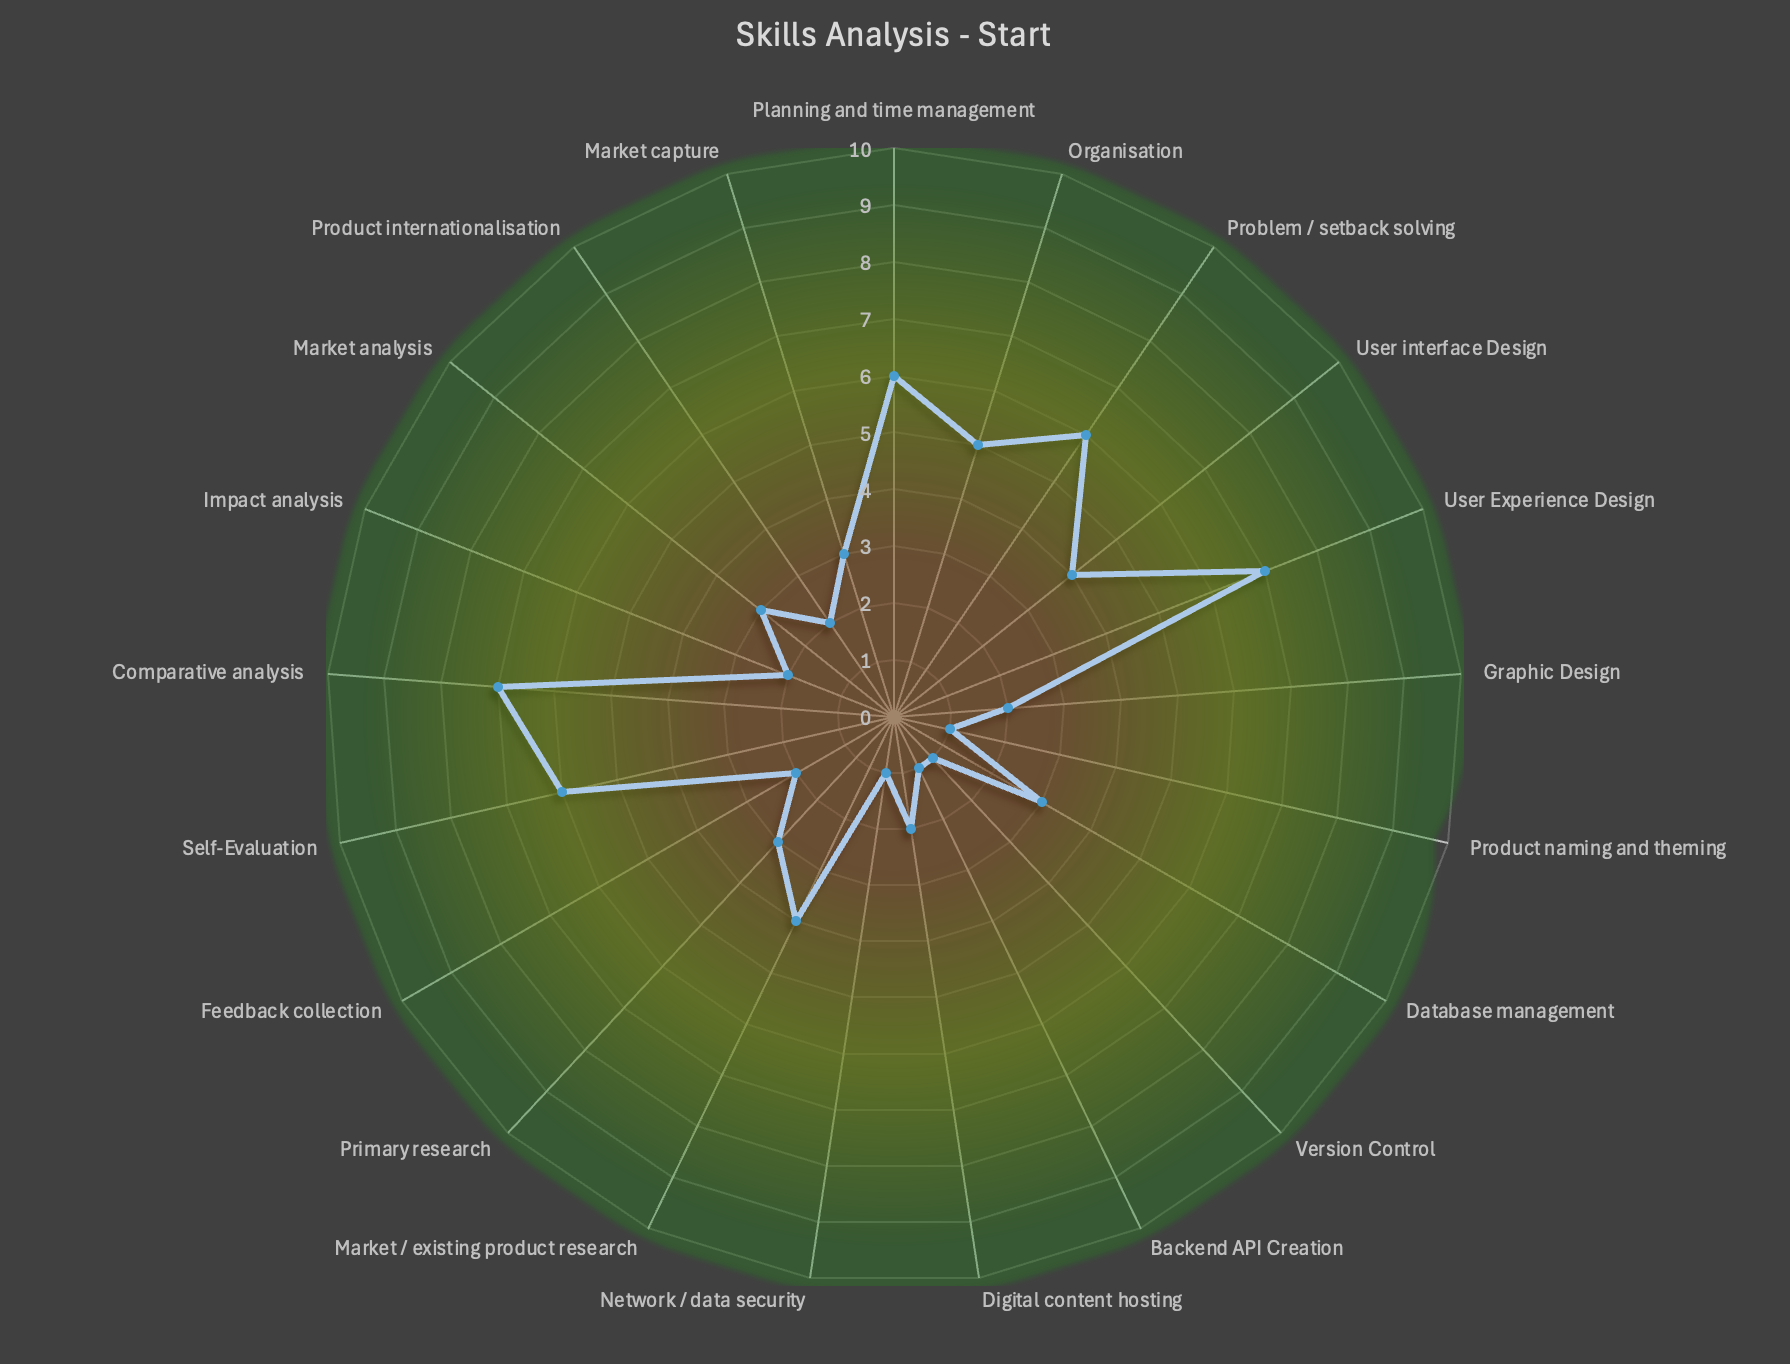
\includegraphics[width=0.8\textwidth]{SkillDevelopment/SkillsAudit/media/initialSkillsAnalysis.png}
    \caption{Initial skills Audit Visualisation}
    \label{fig:SkillsAuditVisualisation}
\end{figure}

\begin{longtable}{
  >{\raggedright\arraybackslash}p{0.4\textwidth}  % First column with fixed width
  >{\centering\arraybackslash}p{1.5cm}  % Middle column has fixed width
  >{\raggedright\arraybackslash}p{0.4\textwidth}  % Third column with fixed width
}
\toprule
\textbf{Skill} & \textbf{Rating?} & \textbf{Explanation / improvement plan} \\
\midrule
\endfirsthead

\multicolumn{3}{c}%
{{\bfseries \tablename\ \thetable{} -- continued from previous page}} \\
\toprule
\textbf{Skill} & \textbf{Rating?} & \textbf{Explanation / improvement plan} \\
\midrule
\endhead

\midrule \multicolumn{3}{r}{{Continued on next page}} \\
\endfoot

\bottomrule
\endlastfoot

\rowcolor{gray!10}
\multicolumn{3}{l}{\textbf{Project Management}} \\ Planning and time management & 4 & My project will start with a number of plans being created regarding progress and timeframes, producing these will grow my skills in these area \\
Organisation  & 5 & The EPQ program requires regular commitment to research, analysis and development which will soon increase my organisational skills\\
Problem \& setback solving & 6 & I'm sure many challenges will arise throughout the creation of my project but these will presents opportunities to learn. \\


\rowcolor{gray!10}
\multicolumn{3}{l}{\textbf{Design Skills}} \\
User interface Design & 4 & I'm going to research various methods of making digital designs accessible and practical to use \\
User Experience Design & 7 & Iterating through my designs with regular peer feedback to help inform future revisions \\
Graphic Design & 2 & Exploring past artistic trends to inform design choices \\
Product naming and theming & 1 & Brainstorming ideas and gaining peer feedback before iterating \\

\rowcolor{gray!10}
\multicolumn{3}{l}{\textbf{Technical Skills}} \\
Typing & 4 & Completing the enrichment typing course on the KAZ portal \\
Database management & 3 & Research into various database technologies and the tools to mange them \\
Version Control & 1 & Building up good programming practice using tools like GIT \\
Backend API Creation & 1 & Building and maintaining data routes by researching best practice \\
Digital content hosting & 2 & Exploring the cost of digital product publishing and upkeep \\
Network \& data security & 1 & Critical elements to get right will require rigorous testing and research into best practices \\

\rowcolor{gray!10}
\multicolumn{3}{l}{\textbf{Research Skills}} \\
Market \& existing product research & 4 & Exploring current note taking applications to learn from their high / low points \\
Primary research & 3 & Conducting surveys and interviews to gather first hand data \\
Feedback collection & 2 & Understanding how to gain the most possible from valuable peer feedback \\

\rowcolor{gray!10}
\multicolumn{3}{l}{\textbf{Evaluation Skills}} \\
Self-Evaluation & 6 & Critiquing oneself to understand areas for improvement \\
Comparative analysis & 7 & Expanding on the self evaluation by understanding how your work compares to others in the same industry \\
Impact analysis & 2 & Understanding the shift you have made in the consumers mind by the introduction of your product \\
Market analysis & 3 & Exploring what the market wants, and how current offering don't fulfil that need \\
\end{longtable}
\subsection{Christmas Re-audit}

\begin{figure}[H]
    \centering
    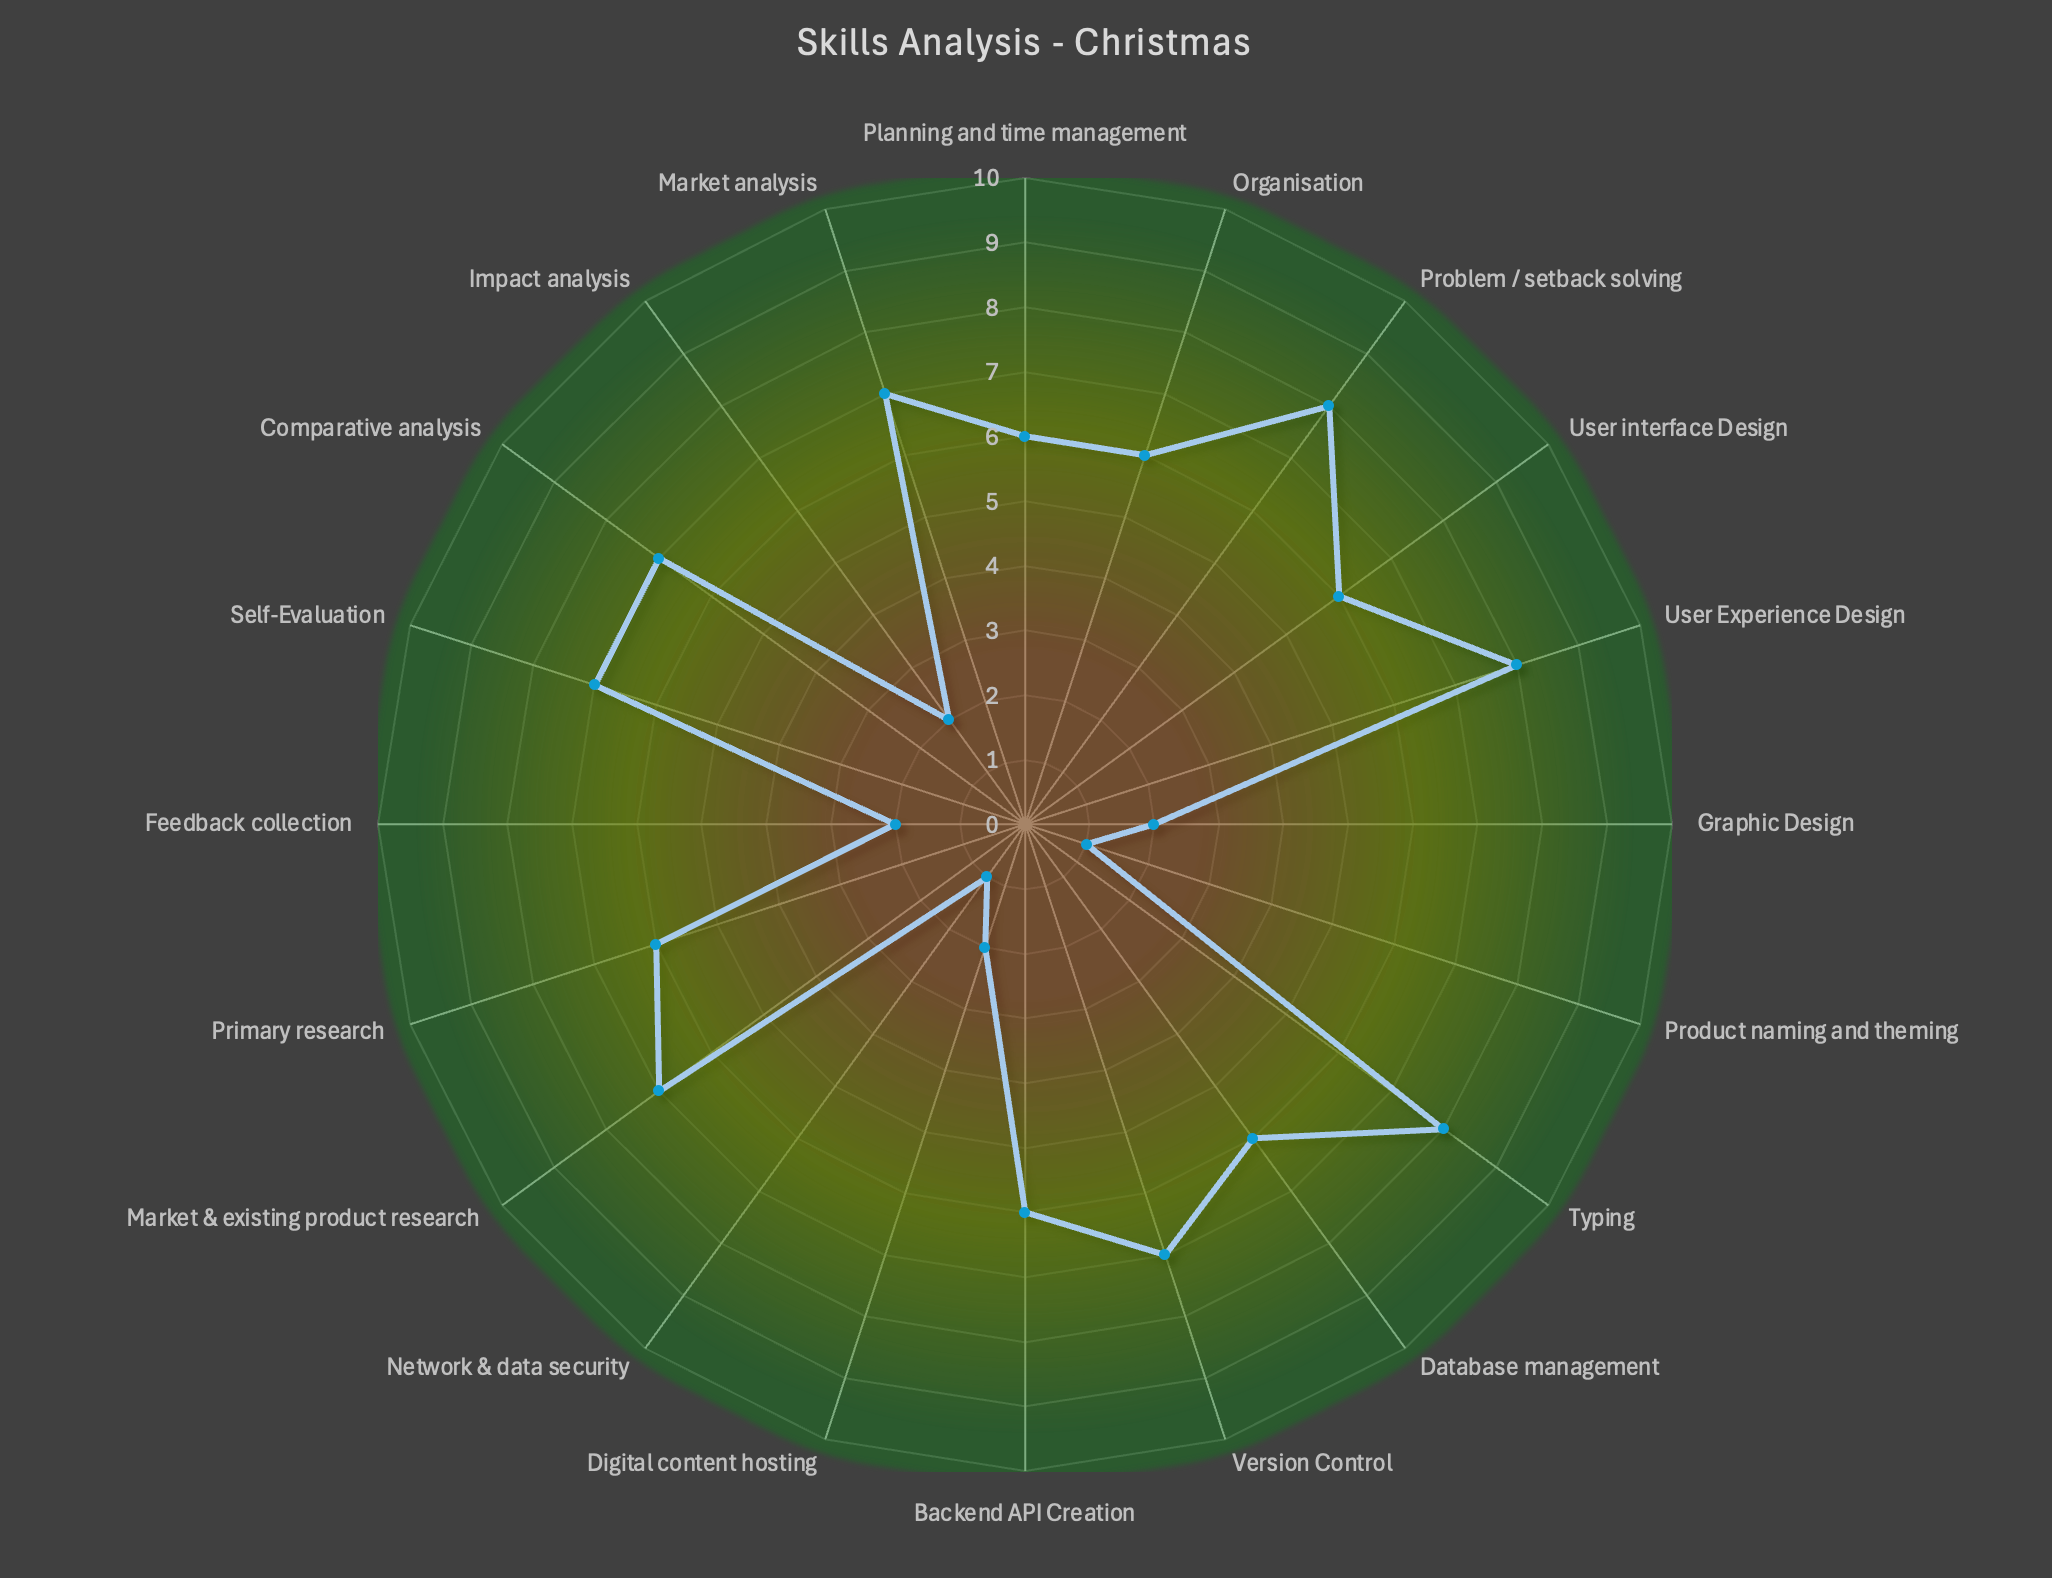
\includegraphics[width=0.8\textwidth]{SkillDevelopment/SkillsAudit/media/analysisChristmas.png}
    \caption{Christmas skills Audit Visualisation}
\end{figure}


\begin{longtable}{
  >{\raggedright\arraybackslash}p{0.4\textwidth}  % First column with fixed width
  >{\centering\arraybackslash}p{1.5cm}  % Middle column has fixed width
  >{\raggedright\arraybackslash}p{0.4\textwidth}  % Third column with fixed width
}
\toprule
\textbf{Skill} & \textbf{Rating?} & \textbf{Explanation / improvement plan} \\
\midrule
\endfirsthead

\multicolumn{3}{c}%
{{\bfseries \tablename\ \thetable{} -- continued from previous page}} \\
\toprule
\textbf{Skill} & \textbf{Rating?} & \textbf{Explanation / improvement plan} \\
\midrule
\endhead

\midrule \multicolumn{3}{r}{{Continued on next page}} \\
\endfoot

\bottomrule
\endlastfoot

\rowcolor{gray!10}
\multicolumn{3}{l}{\textbf{Project Management}} \\ 

Planning and time management & 6 (+2) & My initial timelines and planning have been incredibly helpful to me as I have dived into my project. As I have continually evaluated my progress and time usage I have even found myself ahead of plan and have utilised updated timelines to allocate "new found time" to be used to improve various subsets of my project \\

Organisation & 6 (+1) & Similar to above, I have been careful to stick to the plans and timelines I formed at the beginning of the project and this has really helped me to maintain strong progress without 'burn out' or losing focus \\

Problem \& setback solving & 8 (+2) & Throughout my software development so far I have across many different challenges. Utilising my developing research skills I have found solutions to each and every one of these, enabling me to keep my project plan on track, whilst producing software far beyond my original expectation of quality \\

\rowcolor{gray!10}
\multicolumn{3}{l}{\textbf{Design Skills}} \\ 

User Interface Design & 7 (+3) & I have been able to apply my learnings around user interface design to create a product that is both functional and visually appealing as described in my diary entries and prototypes. I have also received positive feedback from peers on the usability of my designs \\

User Experience Design & 8 (+1) & I have iterated through my designs with regular peer feedback to help inform future revisions, this process has helped me to see features from a variety of features and helps accomodate for the widest variety of users possible. \\

\rowcolor{gray!10}
\multicolumn{3}{l}{\textbf{Technical Skills}} \\ 

Typing & 8 (+4) & I have been able to complete the KAZ typing course and have found myself typing faster and more accurately than ever before, this has been a huge help in my software development as I can now type code faster than I can think of it! I achieved 72WPM on a 'complex' literature challenge (consisting of many less frequently used punctuation marks), and average around 100-110 WPM during more standard tasks \\

Database management & 6 (+3) & I have been able to research various database technologies and the tools to manage them, I have also been able to apply this knowledge to my project by using a SQL database to store user data and application state. Having not really explored the practical side of this task (previously only having gauge knowledge of the theory), it has been very satisfying to operate my own database using just a small Raspberry Pi in my house \\

Version Control & 7 (+6) & I have been able to build up good programming practice using tools like GIT, this has been incredibly helpful in my software development as it has allowed me to track changes and revert to previous versions of my code if needed. I completed a couple of GIT fundamental courses to achieve this knowledge growth which were invaluable \\

Backend API Creation & 6 (+5) & I have been able to build and maintain data routes using Python Flask, this has been a huge help in my software development as it has allowed me to create a robust and scalable backend for my application. I have also been able to apply this knowledge to my project by using a RESTful API to communicate between the frontend and backend of my software \\

\rowcolor{gray!10}
\multicolumn{3}{l}{\textbf{Research Skills}} \\ 

Market \& existing product research & 7 (+3) & As recorded in my research section, I have studied a wide range of currently existing products, both direction 'competition' (Note-taking apps) and software further afield such as project management software which incorporated features I found useful in a different context \\

Primary Research & 6 (+3) & I have conducted surveys and interviews with family, friends and others to gather first-hand data, this has been incredibly helpful in my software development as it has allowed me to understand the needs and wants of my users. \\

\rowcolor{gray!10}
\multicolumn{3}{l}{\textbf{Evaluation Skills}} \\ 

Self Evaluation & 7 (+1) & Throughout my EPQ Journey so far I have been continually re-evaluating to help me set better goals for my self and manage my productivity. This is perhaps the most crucial skill to develop as it has so many benefits further in life \\

Market analysis & 7 (+4) & As mentioned above by exploring the existing product options i have gained a better understanding of the industry my software would sit within \\

\end{longtable}

\subsection{Mid-Project Re-audit}

\begin{figure}[H]
    \centering
    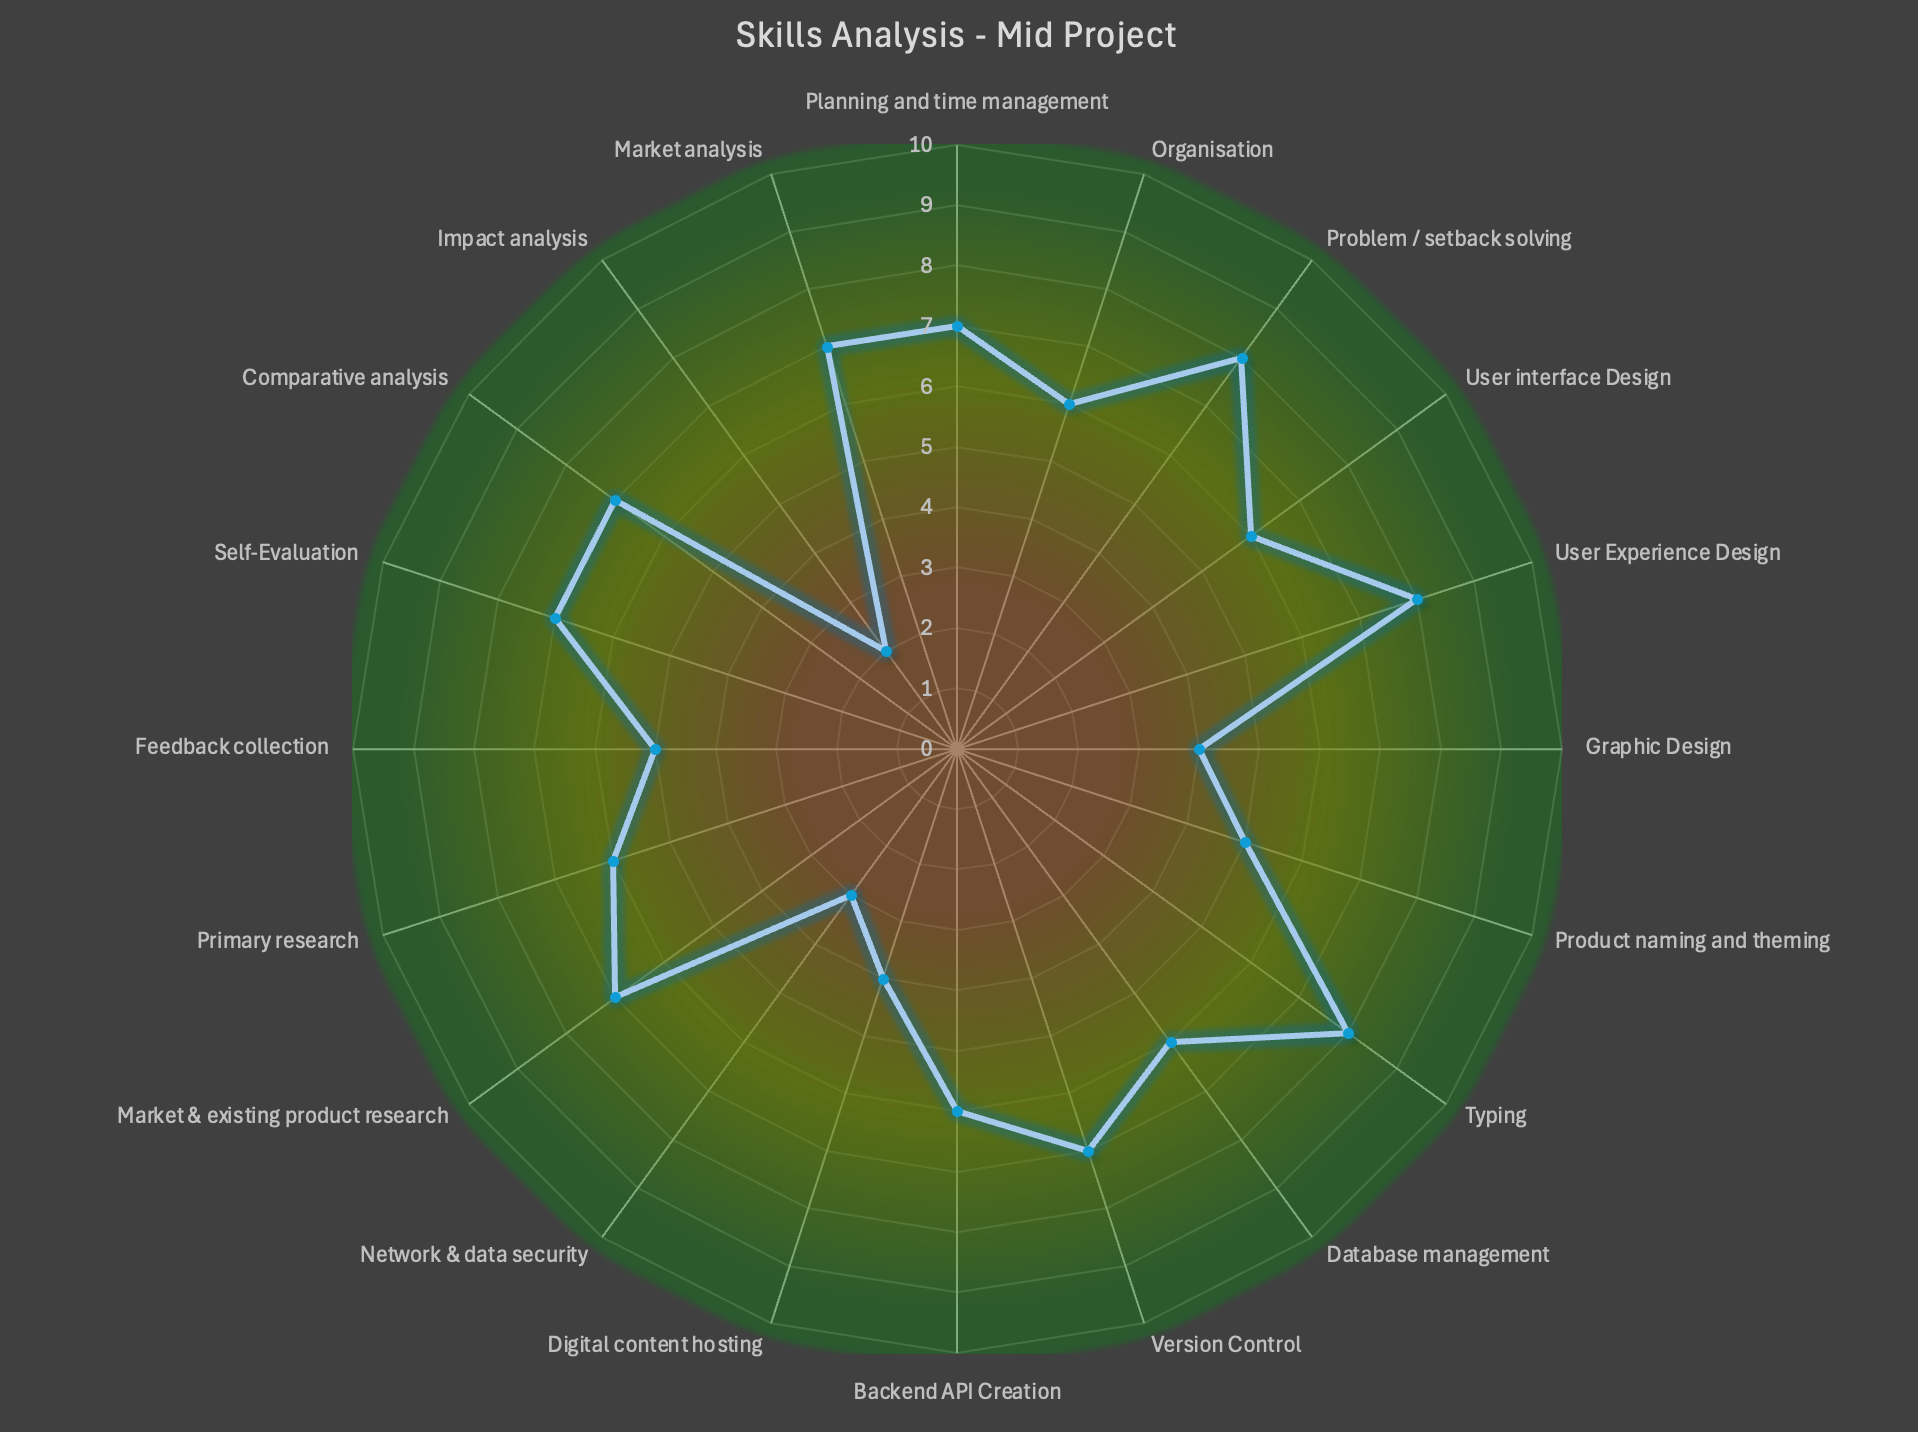
\includegraphics[width=0.8\textwidth]{SkillDevelopment/SkillsAudit/media/analysisMidProject.png}
    \caption{Mid-Project skills Audit Visualisation}
\end{figure}

\begin{longtable}{
  >{\raggedright\arraybackslash}p{0.4\textwidth}  % First column with fixed width
  >{\centering\arraybackslash}p{1.5cm}  % Middle column has fixed width
  >{\raggedright\arraybackslash}p{0.4\textwidth}  % Third column with fixed width
}
\toprule
\textbf{Skill} & \textbf{Rating?} & \textbf{Explanation / improvement plan} \\
\midrule
\endfirsthead

\multicolumn{3}{c}%
{{\bfseries \tablename\ \thetable{} -- continued from previous page}} \\
\toprule
\textbf{Skill} & \textbf{Rating?} & \textbf{Explanation / improvement plan} \\
\midrule
\endhead

\midrule \multicolumn{3}{r}{{Continued on next page}} \\
\endfoot

\bottomrule
\endlastfoot

\rowcolor{gray!10}
\multicolumn{3}{l}{\textbf{Project Management}} \\ 
Planning and time management & 7 (+1) & I have continued to utilise my short and long term plans to guide my progress and have found myself always on track or even ahead of schedule. I have also been able to adapt my plans as needed to accommodate for any unforeseen challenges or opportunities that have arisen \\

\rowcolor{gray!10}
\multicolumn{3}{l}{\textbf{Design Skills}} \\ 
User Interface Design & 7 (+1)& Further iterating on my designs with new colour variations, and improved spacing has enhanced my design skills  \\
Graphic Design & 4 (+2) & By creating some website assets in Adobe Illustrator I have hugely improved my design skills\\
Product naming and theming & 5 (+4) & With a name nearly decided (draft name is NeuroNote) I have explored links ranging from ancient mythology and Norse gods to complex data surrounding the brain to have a name which is both memorable and meaningful\\

\rowcolor{gray!10}
\multicolumn{3}{l}{\textbf{Technical Skills}} \\ 
Digital content hosting & 4 (+2) & Having explored server management on my Raspberry Pi, I now feel much more confidence getting my project fully accessible from anywhere\\
Network \& data security & 3 (+2) & During my EPQ I have learnt about many skills such as Password encryption, and more recently techniques to secure the transfer of data across the internet. These techniques are crucial to any Internet product\\

\rowcolor{gray!10}
\multicolumn{3}{l}{\textbf{Research Skills}} \\ 
Feedback collection & 5 (+3) & Since Christmas I have utilised and assessed many more resources which have all helped me build a robust understanding of how to determine the validity of a source\\
\end{longtable}

\subsection{Easter Re-audit}

\begin{figure}[H]
    \centering
    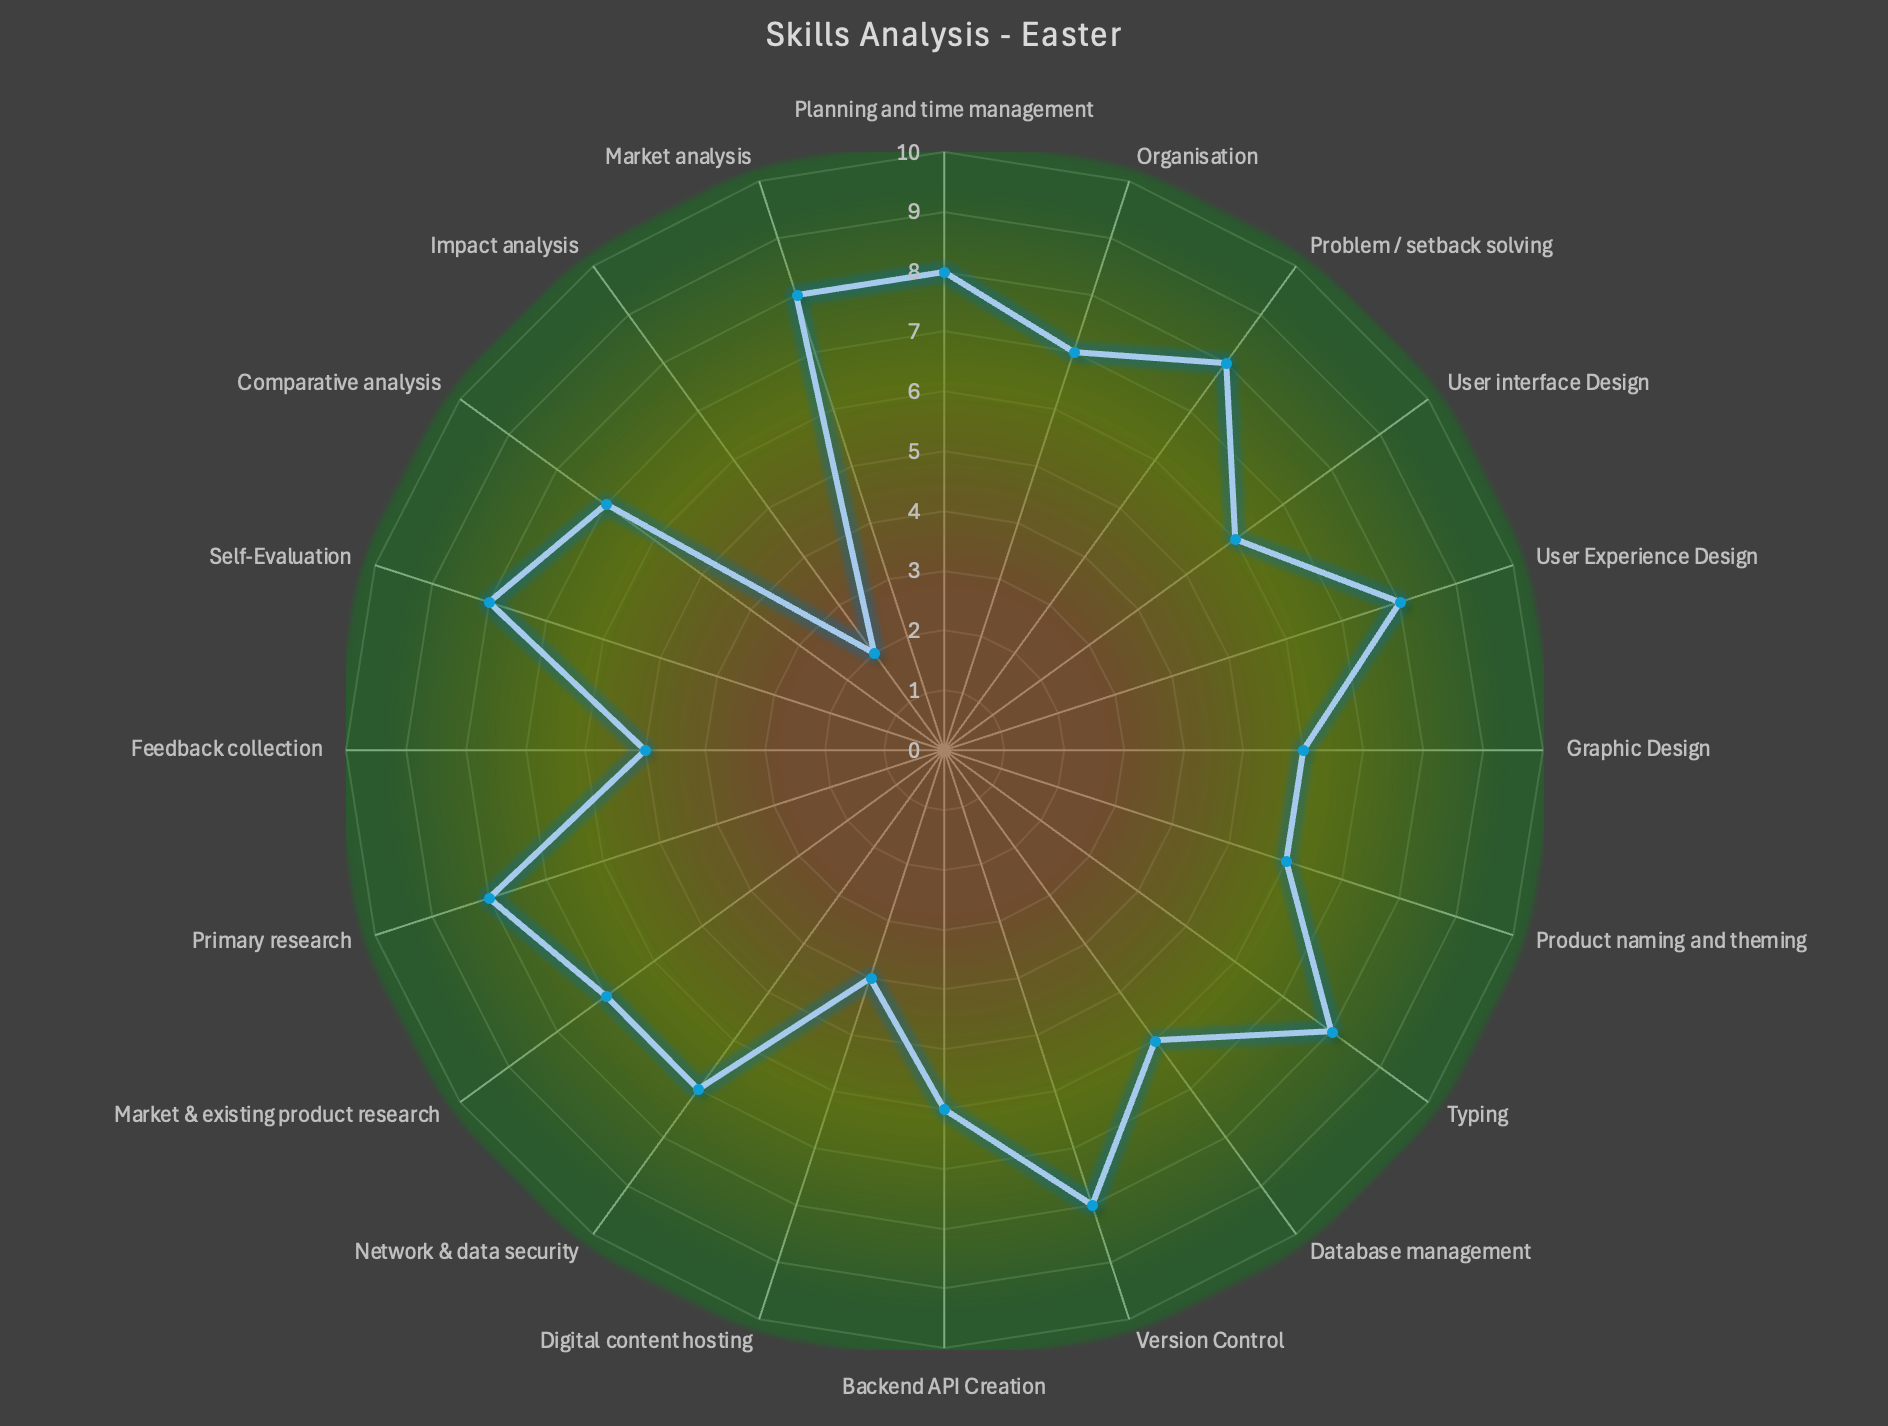
\includegraphics[width=0.8\textwidth]{SkillDevelopment/SkillsAudit/media/analysisEaster.png}
    \caption{Easter skills Audit Visualisation}
\end{figure}

\begin{longtable}{
  >{\raggedright\arraybackslash}p{0.4\textwidth}  % First column with fixed width
  >{\centering\arraybackslash}p{1.5cm}  % Middle column has fixed width
  >{\raggedright\arraybackslash}p{0.4\textwidth}  % Third column with fixed width
}
\toprule
\textbf{Skill} & \textbf{Rating?} & \textbf{Explanation / improvement plan} \\
\midrule
\endfirsthead

\multicolumn{3}{c}%
{{\bfseries \tablename\ \thetable{} -- continued from previous page}} \\
\toprule
\textbf{Skill} & \textbf{Rating?} & \textbf{Explanation / improvement plan} \\
\midrule
\endhead

\midrule \multicolumn{3}{r}{{Continued on next page}} \\
\endfoot

\bottomrule
\endlastfoot

\rowcolor{gray!10}
\multicolumn{3}{l}{\textbf{Project Management}} \\ 
Planning and time management & 8 (+1) & I have continued to utilise my plans and more specific task sheets to maximise my productivity\\

organisation & 7 (+1) &  I have refined many of diary entries formatting and research pieces to more clearly lay out my next steps and identify and weak points in my topic knowledge\\

\rowcolor{gray!10}
\multicolumn{3}{l}{\textbf{Design Skills}} \\
Graphic Design & 6 (+2) & I have continued designing some assets for my platform such as welcome screens and banners\\
Product naming and theming & 8 (+3) & Continuing to build on my product theming with a variety of colours placed around my User Interface to signal 'danger' areas and information \\

\rowcolor{gray!10}
\multicolumn{3}{l}{\textbf{Technical Skills}} \\
Version Control & 8 (+1) & I have continued to follow Version control best practices through the use of various 'branches' to implement features within my project \\
Network \& data security & 7 (+4) & \\

\rowcolor{gray!10} 
\multicolumn{3}{l}{\textbf{Research Skills}} \\
Primary research & 8 (+2) & I have continued speaking to my peers and sending round various iterations of my prototypes to gauge which would be most useful to my users \\

\rowcolor{gray!10}
\multicolumn{3}{l}{\textbf{Evaluation Skills}} \\
Self Evaluation & 8 (+1) & My diary continues to evaluate my ongoing progress \\
Market analysis & 8 (+1) & I have continued to explore various competitors (such as OneNote) throughout my studies when required to. Using NeuroNote whenever I have the opportunity\\

\end{longtable}


\subsection{End of Project Audit}

\begin{figure}[H]
    \centering
    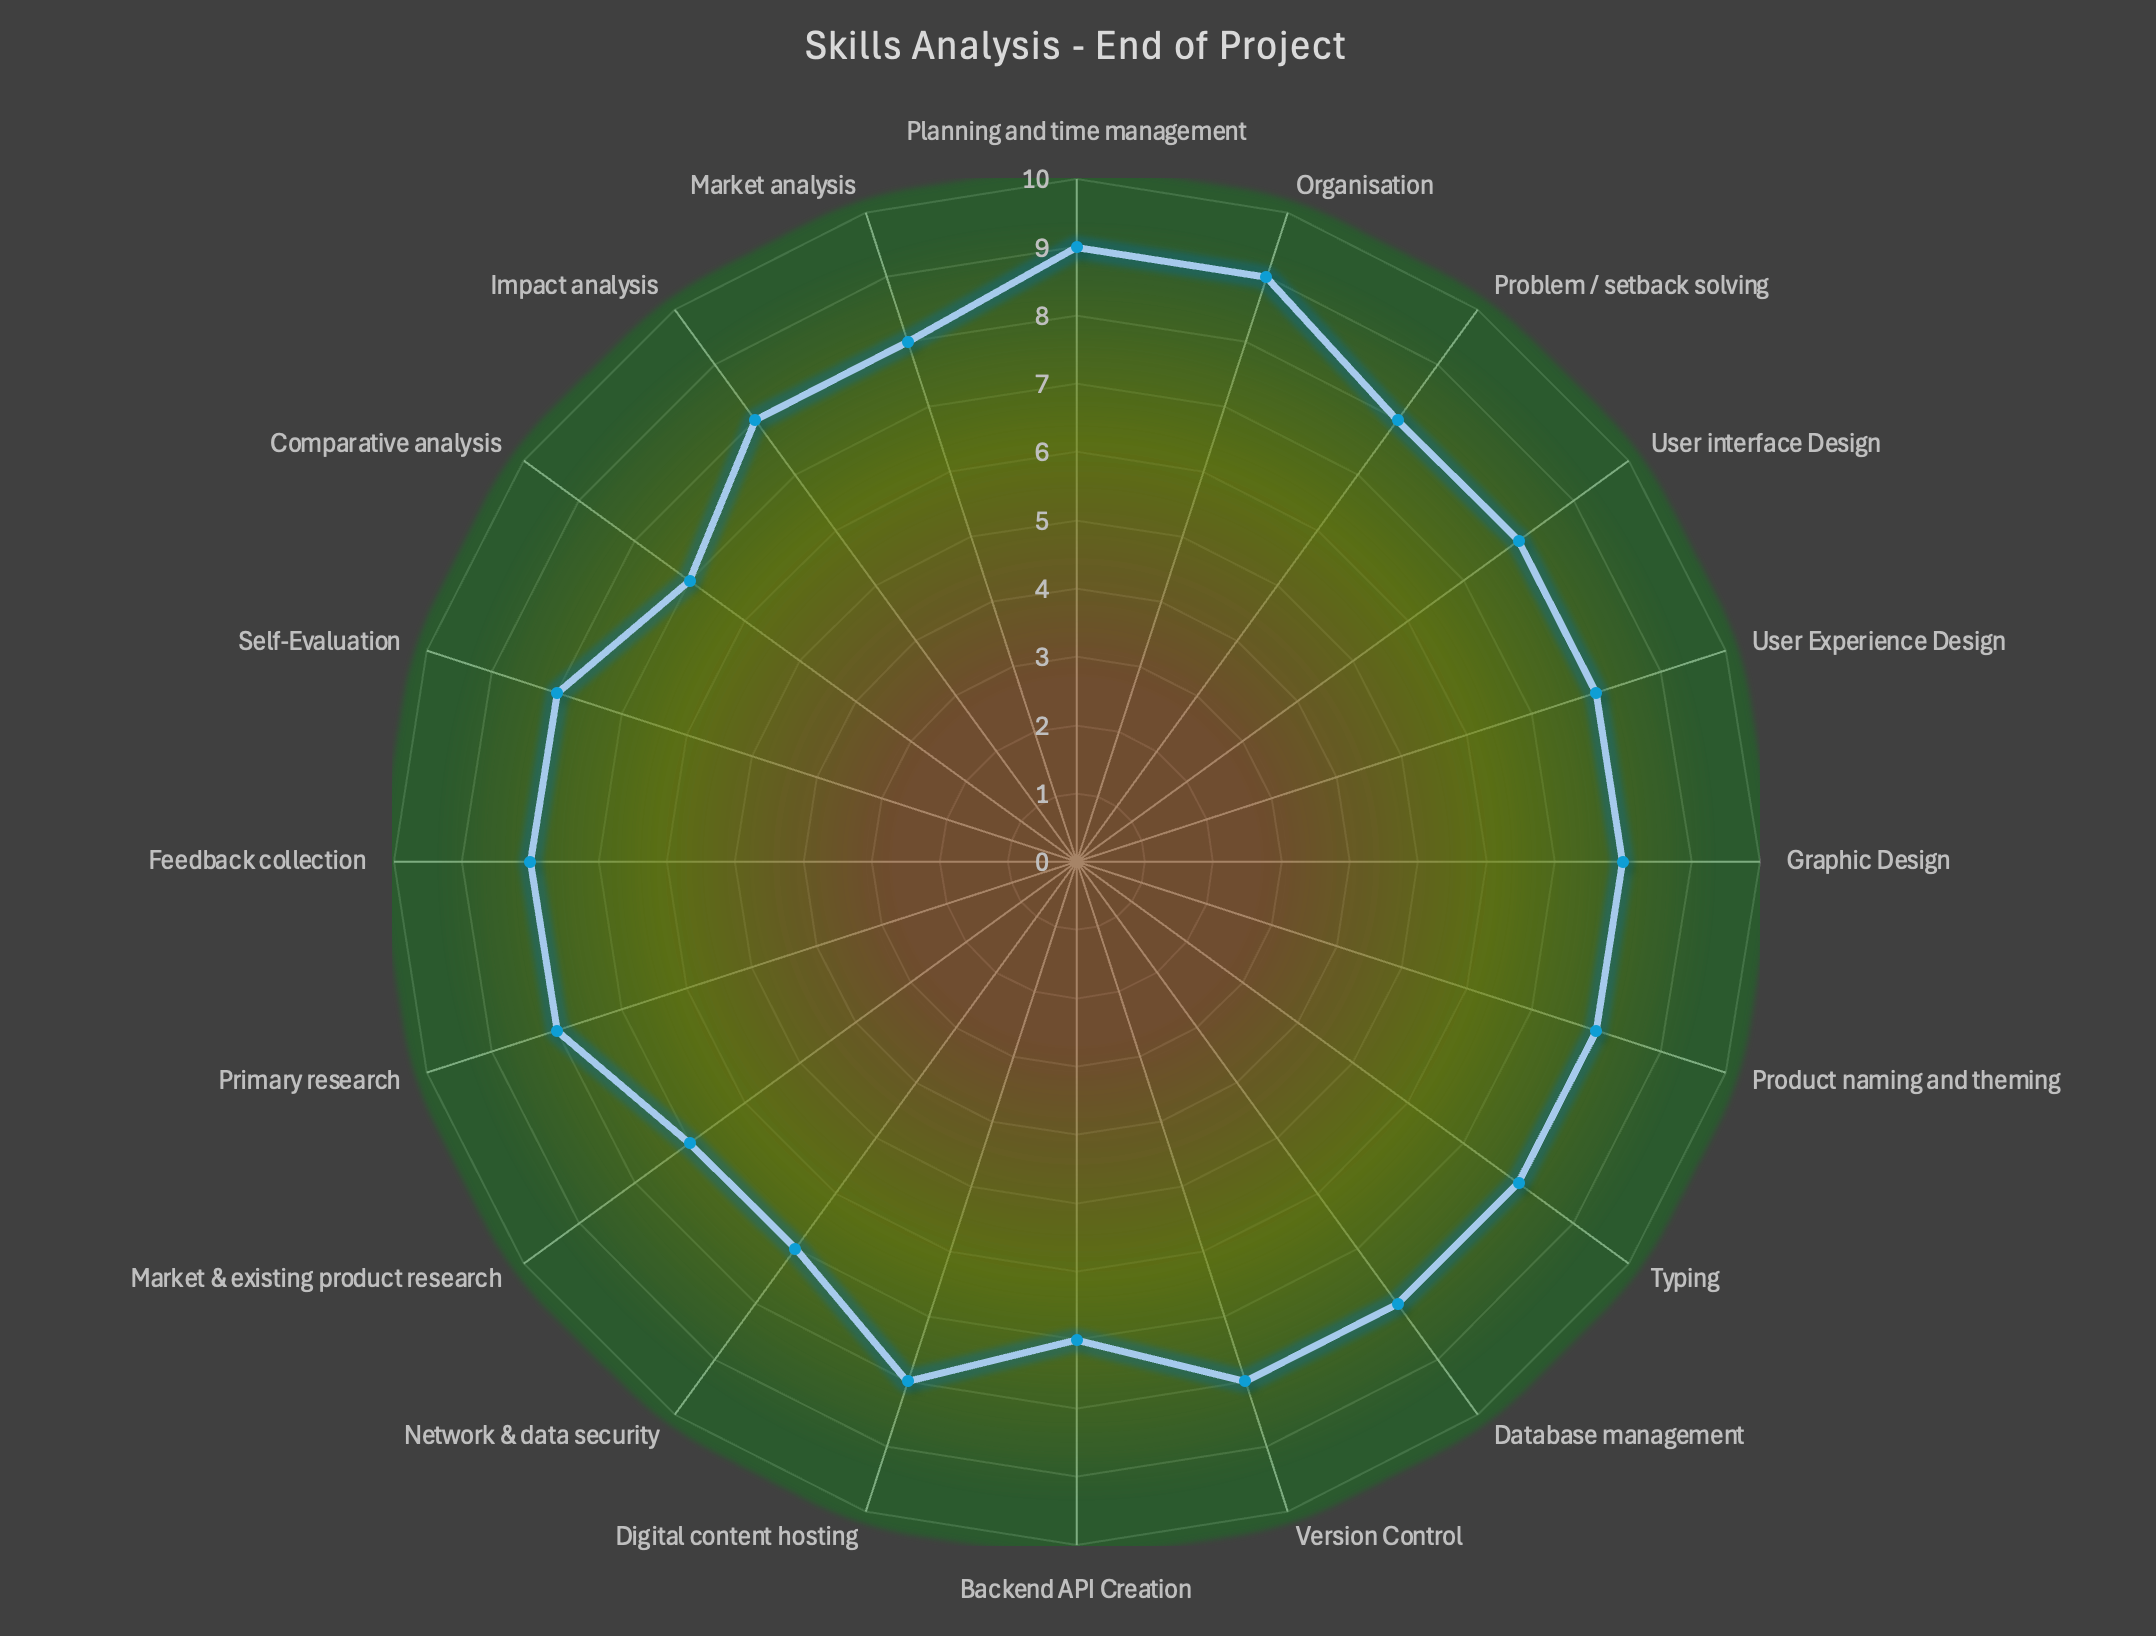
\includegraphics[width=0.8\textwidth]{SkillDevelopment/SkillsAudit/media/analysisEnd.png}
    \caption{End of Project skills Audit Visualisation}
\end{figure}

\begin{longtable}{
  >{\raggedright\arraybackslash}p{0.4\textwidth}  % First column with fixed width
  >{\centering\arraybackslash}p{1.5cm}  % Middle column has fixed width
  >{\raggedright\arraybackslash}p{0.4\textwidth}  % Third column with fixed width
}
\toprule
\textbf{Skill} & \textbf{Rating?} & \textbf{Explanation / improvement plan} \\
\midrule
\endfirsthead

\multicolumn{3}{c}%
{{\bfseries \tablename\ \thetable{} -- continued from previous page}} \\
\toprule
\textbf{Skill} & \textbf{Rating?} & \textbf{Explanation / improvement plan} \\
\midrule
\endhead

\midrule \multicolumn{3}{r}{{Continued on next page}} \\
\endfoot

\bottomrule
\endlastfoot

\rowcolor{gray!10}
\multicolumn{3}{l}{\textbf{Project Management}} \\ 


Planning and time management & 9 (+1) & As I have brought my project to a close I have completed all of my goals in addition to many 'stretch targets' I set out for myself along the way\\
organisation & 9 (+2) & I have successfully launched my project to a wide range of users which required maintaining a lot of technical infrastructure and replying to users who had questions, feedback or technical issues\\

\rowcolor{gray!10}
\multicolumn{3}{l}{\textbf{Design Skills}} \\ 

Graphic Design & 8 (+2) & Within my project presentation I created many assets such as a 3d Animated logo intro. This drew on some pre-existed skills but enabled me to integrate my graphical design exploration throughout my project to make a visually appealing product \\

\rowcolor{gray!10}
\multicolumn{3}{l}{\textbf{Technical Skills}} \\ 

Database management & 8 (+2) & With over 100 users accessing my platform I made use of robust database backups and controls. I additionally had to use 'database rollbacks' to aid users who had internally overwritten content \\
Backend API Creation & 7 (+1) & I was very pleased to see that my infrastructure held up to my product launch's demand. Overall I have only had to make a few small changes (such as allowing requests to be handled my multiple Raspberry Pi's not just one) and my users have been very satirised with platform performance and latency \\
Digital Content Hosting & 8 (+4) & Bringing my Project operational and accessible across the globe has taught me so many key skills such as Reverse Proxies, Website Certifications and Cross Origin Resource Sharing (CORS - which helps a backend system identify where a request has originated from in order to reduce fraud / unauthorised access) \\


\rowcolor{gray!10}
\multicolumn{3}{l}{\textbf{Evaluation Skills}} \\ 
Feedback collection & 8 (+3) & After the announcement of my product launch I pointed my users towards a feedback form within my platform. I custom-made this feedback portal, and it has enabled me to gain a much greater insight into the opinions of my user base\\
Self-Evaluation & 9 (+1) &  Following from this research I completed my final project evaluation which took the context of my entire EPQ and reflected upon the success of each element\\
Impact analysis & 8 (+6) & With such an incredible reception to my launch I was able to use metrics such as page visit time, user count and the feedback forms submitted to establish how my product could fit within the larger industry. This skill is frequently used within a professional software development team to better understand not just the market they are launching into but how they can expand to other related industries. \\

\end{longtable}

